%&LaTeX

\section{The Matlab Lab, or How to Not Teach a Programming Language}

Labs in this class will make liberal use of the Matlab numerical
programming environment. Because this class assumes that you are an
experienced computer science student, you are expected to be able to
learn how to use computer tools, and how to program in new programming
languages, pretty much on your own. So, the first thing you should do
is check out the Matlab documentation built into the Matlab help
system, or online at
\url{http://www.mathworks.com/help/matlab/index.html}. Of course, you
can always search online for Matlab tutorials and the like. We'll
include a very brief overview of Matlab below, and then more detailed
information about the code developed specifically for this class that
you will be using.

\subsection{Matlab in a (Very Small) Nutshell}
\label{sc:basic-matlab}

The Matlab GUI environment is very similar to IDEs that you are
already familiar with. As you might expect, there are some
idiosyncrasies here and there, but nothing terribly unexpected. The
major areas of difference are tools and panes that have to do with
viewing variables (something in other IDEs that you'd only see when
debugging a program), the command pane, and figure windows that open
to display graphs. The first two of these differences have to do with
the fact that Matlab is an interpreted language/programming
environment. You primary area of interaction with the Matlab
interpreter will be through the command window, with variable
information panes providing views of variables and their contents
related to your interaction. It's interesting to note that, if you
want, you can run Matlab without the GUI, providing just a command
line interface.

Interpreted languages have their advantages and disadvantages.  One
advantage is that anything you can use as a line of code in a program
you can use immediately as a command on the command line. This lets
you test code interactively and then copy it into the script or
function you're writing. Like any IDE, Matlab includes an editor with
syntax highlighting and debugger integration.

The disadvantage is the interpreted programs are slower. In Matlab, we
get around this by using built-in functions that operate on entire
vectors or arrays as single data objects. The core loops of the
built-in functions are compiled for speed. If you make good use of
those functions, Matlab code can often be as fast as completely
compiled code.

Here are some things to try:
\begin{enumerate}
\item Immediate calculations and variables:
\begin{verbatim}
   radius = 5    % Comments start with "%"
   circumference = 2 * pi * radius
   area = pi * radius^2
\end{verbatim}
\item Complex numbers:
\begin{verbatim}
   sqrt(-1)
   x = 7 + 14j
   conj(x)       % complex conjugate
   abs(x)        % magnitude (e.g., for polar representation)
   angle(x)      % and angle for polar rep
   real(x)
   imag(x)
\end{verbatim}
\item Complex exponentials:
\begin{verbatim}
   exp(j * pi)
   exp(j * pi/2)
   exp(j * pi/4)
\end{verbatim}
\item Vectors:
\begin{verbatim}
   v1 = [0 1 2 3]    % Four elements
   v2 = [0 : 2 : 10] % like a loop (start value : increment : end value)
   v3 = pi * [-0.5 -0.25 0 0.25 0.5] % All operations are vectorized
   exp(j * v3)
   mistake = v1 * v1     % a mistake; vector mult doesn't work this way
   dotproduct = v1 * v1' % transposing will work, if you want to do this
   arrayprod = v1 .* v1  % element-by-element ops include: .+, .-, .*, ./
\end{verbatim}
\item Simple plots (note that ``;'' suppresses outputting results to
  the command window --- useful if that would generate massive amounts
  of text, or just if you want things neat):
\label{it:simple-plots}
\begin{verbatim}
   t = [0 : 0.01 : 2*pi];
   x = sin(t);
   plot(t, x);       % default plots points connected by lines in blue
   plot(t, x, 'r');  % change the line color
   plot(t, x, 'r.'); % change the plot style; zoom in to see individual points
   xlabel('t, ms');  % X axis label (all of your plots should have this)
   ylabel('Mag');    % Y axis label (all of your plots should have this)
   title('Triangle');% Graph title (all of your plots should have this)
\end{verbatim}
\end{enumerate}

If you take a sequence of commands and save them in a file with an
extension of \texttt{.m}, the result is a \emph{script}. Assuming that the
script is saved in a directory in the MATLAB search path, you can then
execute the script by just typing its name (without the \texttt{.m}),
just as if it were a command. If you want your code to take
parameters, return a return value, and have local variables, start
your code with a line like:
\begin{verbatim}
   function retval = funcname(parm1, parm2)
\end{verbatim}
Your code is now a function. MATLAB functions can take variable
numbers of arguments and even return variable numbers of return
values, but that's getting beyond what we need right now.

\paragraph{Step 1.1} Extracting and/or inserting numbers in a
vector is very easy to do. Consider the following definition:
\begin{verbatim}
   x = [ ones(1,4), [2:2:11], zeros(1,3) ]
   x(3:7)
   length(x)
   x(2:2:length(x))
\end{verbatim}
Explain the result echoed from the last three lines of the above code.

\paragraph{Step 1.2} In the previous step, the vector \texttt{x}
contained 12 elements. Observe the result of the following assignment:
\begin{verbatim}
   x(3:7) = pi*(1:5)
\end{verbatim}
Now write a statement that will replace the odd-indexed elements of
\texttt{x} with the constant -77 (i.e., \texttt{x(1)},
\texttt{x(3)}, etc). Use vector indexing and vector replacement.


\paragraph{Step 1.3} Vectorization is an essential programming
skill in Matlab. Loops can be done in Matlab, but they are not the
most efficient way to get things done. It's better to avoid loops and
use the vector notation instead. For example, the code below uses a
loop to compute values of the sine function. Rewrite this computation
without using the loop (as in list item~\ref{it:simple-plots} in
this section).
\begin{verbatim}
   x = [ ];                  % initialize the x vector to a null
   for k=0:7,
      x(k+1) = sin( k*pi/4 ) % x(0) would fail
   end
x
\end{verbatim}

While thinking this way isn't essential in this course (the loop will
still get the job done), it's probably a valuable skill to learn, as
software moves more and more towards taking advantage of multiple
processors. In this case, \texttt{[0:7]} creates a vector of the
values we want, the scalar multiplication \texttt{*pi/4} generates the
vector of inputs for the \texttt{sin()} function, and the function
itself is vectorized (can take a vector as an input argument) and
returns an equal-sized vector of its results, which are in turn
assigned to \texttt{x}.}

\paragraph{Step 1.4} Consider the following code that plots a
sinusoid:
\begin{verbatim}
   t = [0 : 0.01 : 1]; % time in seconds
   f = 5;              % freq in Hertz
   x = sin(2*pi*f*t);
   plot(t, x);
   xlabel('Time (sec)');
\end{verbatim}
Use the MATLAB editor to create a script file called
\texttt{firstsin.m}, verify that you've saved it in a directory in the
MATLAB path (or add that directory to the path), and test its
execution by typing \texttt{firstsin} at the MATLAB command
prompt. Note that you can also do:
\begin{verbatim}
   type firstsin   % prints out contents of the script
   which firstsin  % shows directory (useful when your code shadows built-ins)
\end{verbatim}

Add three lines of code to your script, so that it will plot a cosine
on top of the sine in a different color. Use the \texttt{hold}
function to add a plot of
\begin{verbatim}
   0.5*cos(2*pi*f*t)
\end{verbatim}
to the plot. See \texttt{help hold} in MATLAB. Enter the three lines
of code you added below. Save the plot using the MATLAB \texttt{print}
command as a JPEG file named \texttt{step14.jpg} by typing:
\begin{verbatim}
   print -djpeg step14
\end{verbatim}
You should include all plots in your lab report, following the
instructions in the report rubric.


\paragraph{Step 1.5} Now generate a tone (i.e., a sinusoid) in MATLAB
and listen to it with the \texttt{sound} command. The frequency of
your tone should be 2 kHz and the duration should be 1 sec. The
following lines of code should be saved in a file called
\texttt{mysound.m} and run from the command line:
\begin{verbatim}
   dur = 1.0;
   f = 2000;
   fs = 8000;
   t = [0 : (1/fs) : dur];
   x = sin(2*pi*f*t);
   sound(x, fs)
\end{verbatim}
The sound hardware will convert the vector of numbers \texttt{x} into
a sound waveform at a certain rate, called the sampling rate (we will
learn a lot more about this in this class). In this case, the sampling
rate is 8000 samples/second, but other values might be used depending
on the capability of sound hardware. What is the length of the vector
\texttt{x}?

\paragraph{Step 1.6} Write a new function that performs the same task
as the following function without using a \texttt{for} loop. Use the
idea in step~1.3 and also consult the section on vector logicals in
the MATLAB documentation. In addition, the MATLAB logical operators
are summarized via \texttt{help relop}.
\begin{verbatim}
   function Z = replacez(A)
   %REPLACEZ Function that replaces the negative elements
   % of a matrix with the number 77
   % usage:
   % Z = replacez(A)
   % A = input matrix whose negative elements are to
   % be replaced with 77
   %
   [M,N] = size(A);
   for i=1:M
      for j=1:N
         if A(i,j) < 0
            Z(i,j) = 77;
         else
            Z(i,j) = A(i,j);
         end
      end
   end
\end{verbatim}


\subsection{Trigonometric Functions and Complex Mathematics in Matlab}


\paragraph{Step 2.1} In this step, you are asked to complete a MATLAB
function to synthesize a waveform in the form of:
\begin{equation*}
x(t) = \sum_{k=1}^N \cos(2\pi f t + \phi_k)
\end{equation*}
This is a sum of cosines, all at the same frequency but with different
phases.  Use the following function prototype to start you off:
\begin{verbatim}
   function x = sumcos(f, phi, fs, dur)
   %SUMCOS Function to synthesize a sum of cosine waves
   % usage:
   % x = sumcos(f, phi, fs, dur)
   %     Returns the sum of cosines at a single frequency f, sampling
   %     rate fs, and duration dur, each with a phase phi.
   % f = frequency
   % phi = vector of phases
   % fs = the sampling rate in Hz
   % dur = total time duration of signal
\end{verbatim}

Include your code in your writeup. Additionally, include a plot of
\texttt{x = sumcos(20, [0 pi/4 pi/2 3*pi/2], 200, 0.25);} versus
time.

Hint: the MATLAB \texttt{length} function is useful in determining the
number of elements in a vector.


\paragraph{Step 2.2} Now, let's see how complex exponentials can
simplify things. Re-implement your \texttt{sumcos} function using
complex exponentials. Take advantage of the fact that multiplying a
complex sinusoid $e^{j2\pi f t}$ by $e^{j\phi}$ will shift its
phase. Thus, you should be able to create a \emph{single} complex
sinusoid at the given frequency \texttt{f} and then multiply it by
\texttt{exp(j * phi)} to get multiple phase shifted cosines. Remember
that we want a real value to plot; the cosine is the real part of a
complex sinusoid. Include your code in your writeup.


\paragraph{Step 2.3} Generate four sinusoids with the following
amplitudes and phases:
\begin{align}
x_1(t) &= 5 \cos(2\pi(15)t +0.5\pi) \\
x_2(t) &= 5 \cos(2\pi(15)t - 0.25\pi) \\
x_3(t) &= 5 \cos(2\pi(15)t +0.4\pi) \\
x_4(t) &= 5 \cos(2\pi(15)t - 0.9\pi) 
\end{align}

\begin{enumerate}\renewcommand{\theenumi}{\alph{enumi}}
\item Make a single plot of all four signals together over a range of
  $t$ that will exhibit approximately 3 cycles. Make sure the plot
  includes negative time so that the phase at $t = 0$ can be
  measured. In order to get a smooth plot make sure that your have at
  least 20 samples per period of the wave. Include your plot in your
  writeup.

\item Verify that the phase of all four signals is correct at $t = 0$,
  and also verify that each one has the correct maximum amplitude. Use
  \texttt{subplot(3,2,i)} to make a six-panel subplot that puts all of
  these plots on the same page, with space for two additional plots at
  the bottom.

\item Create the sum sinusoid,
  $x_5(t)=x_1(t)+x_2(t)+x_3(t)+x_4(t)$. Make a plot of $x_5(t)$ over
  the same range of time as used in the last plot. Include this as the
  lower left panel in the plot by using
  \texttt{subplot(3,2,5)}. Include your plot in your writeup (yes, one
  panel of the figure isn't used).

\item Now do some complex arithmetic; create the complex amplitudes
  corresponding to the sinusoids $x_i(t)$: $z_i = A_ie^{j\phi_i}$,
  $i=1,2,3,4,5$. Print out the $z_i$ in polar and rectangular form,
  showing $A_i$, $\phi_i$, $\Real\{z_i\}$, and $\Imag\{z_i\}$.
\end{enumerate}


\subsection{Representing Analog, Discrete, and Digital Signals}

In our class, we will need to manipulate analog signals (real-valued
signals that are functions of continuous time), discrete signals
(real-valued signals that are functions of discrete time), and digital
signals (discrete-valued signals that are functions of discrete
time). No need to worry about the details or these; that will become
clear later. The trickiest part of this is representing anything other
than digital signals on a digital computer, because you can't. So,
we'll need to employ two key elements of software design: information
hiding and make-believe.

\begin{figure}
\begin{center}
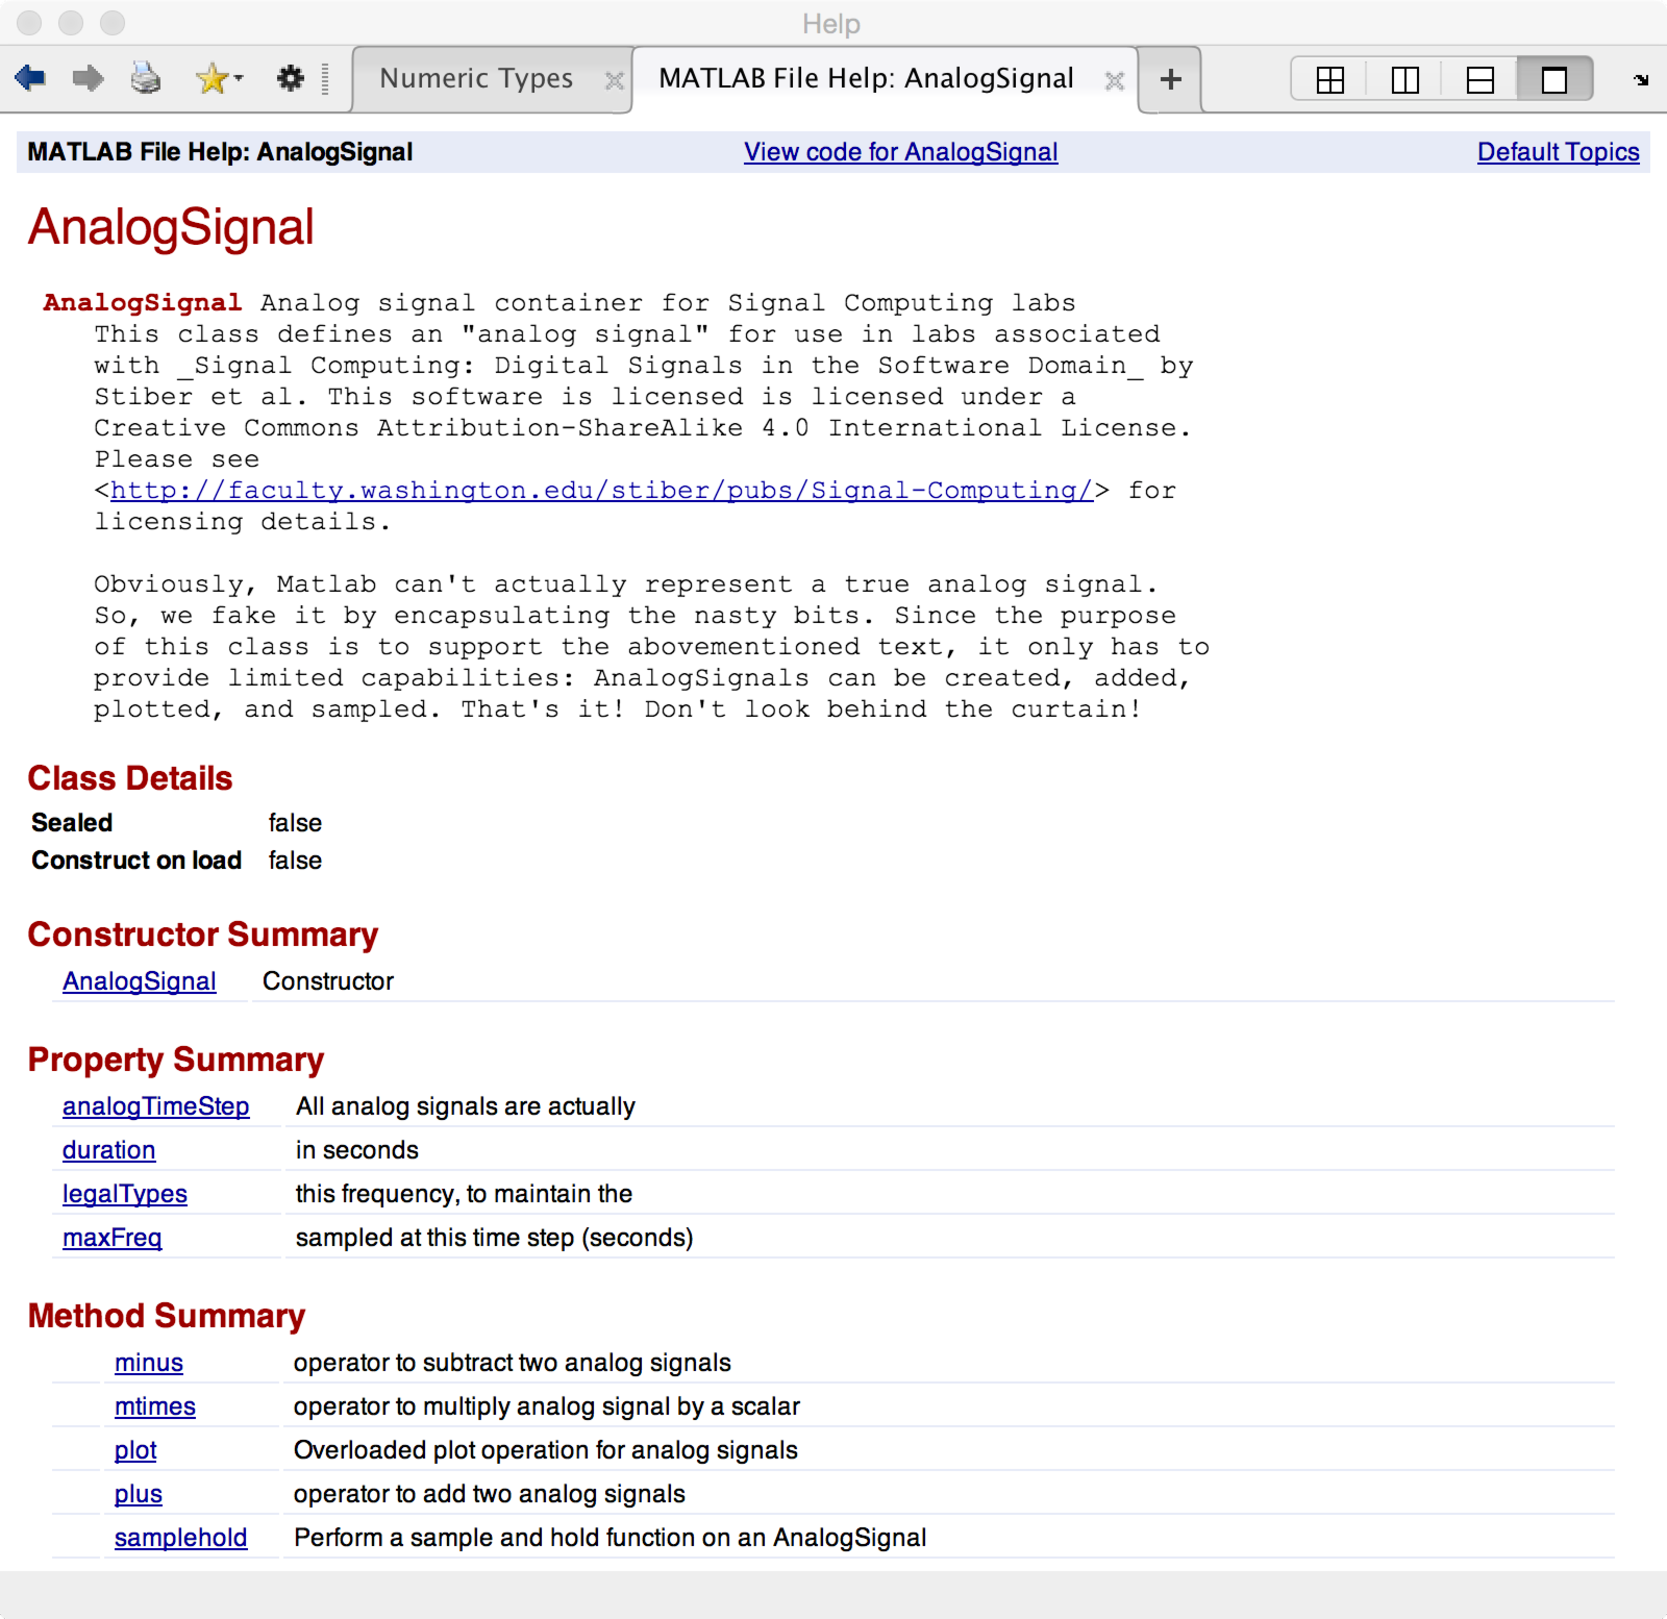
\includegraphics[width=0.75\textwidth]{lab1/AnalogSignal-help}
\end{center}
\caption{.\label{fg:analogsignal-help}}
\end{figure}

Information hiding is used in our implementation of analog signals. We
make use of the object-oriented programming aspects of Matlab to
create an \texttt{AnalogSignal} class. If you look up the documentation
for \texttt{AnalogSignal} (using \texttt{doc AnalogSignal}), you'll
see something like figure~\ref{fg:analogsignal-help}. The key
operations on these analog signals are:
\begin{itemize}
\item Creating an analog signal (ex: \texttt{a =
    AnalogSignal('sawtooth', 2.0, 1.0, 10.0)}).
\item Scaling an analog signal (ex: \texttt{b = a * 5})
\item Adding two analog signals (ex: \texttt{c = a + b})
\item Subtracting two analog signals (ex: \texttt{d = c - a})
\item Plotting an analog signal (ex: \texttt{plot(d)})
\item Sampling an analog signal (ex: texttt{x = d.samplehold(0.1)})
\end{itemize}

You will get a lot more experience working with analog signals shortly
in this class, so for the time being just play with this a bit.

